% Provenance (never printed): see sources/outline_sources.md (Year 3:
% spectral signatures; optical, thermal and radar sensors; radar
% interferometry; digital elevation models; GIS operations).
% Brief: sources/book5/BRIEFS.md, ch. 25. Curves from figdata/bachelor-3/
% spectral_signatures.py (ECOSTRESS spectra and the Landsat 8 OLI bands),
% thermal_ir.py (Planck's law, brightness temperatures, a mixed pixel),
% insar_mogi.py (the wrapped interferogram of a Mogi source) and
% varden_gis.py (slope, aspect and an overlay on the Varden Hills, from
% figdata/shared/region.py, read only). Exercise and problem values in the
% Book 5 scratch calculator calc/ch25.py. Mount Halvren, its lava flows and
% its fumaroles are invented. The brief's overlay (slope > 15 degrees on
% limestone within 200 m of the river) is empty on the Varden model: the
% valley floor is flat; the printed overlay uses the shale within 1 km.
\chapter{Sensoriamento remoto e SIG}\label{ch:b3:remote-sensing-gis}

Em 1997, o solo de uma região selvagem da Cordilheira das Cascatas, perto do conjunto de
vulcões chamados Três Irmãs, começou a se elevar. Em 2001, seu centro estava
\qty{15}{cm} mais alto. Nenhum vulcão se ergue diretamente acima do abaulamento, e a
última erupção da área ocorreu há 1500 anos. O soerguimento não foi percebido por
ninguém caminhando sobre ele: apareceu como um alvo de anéis coloridos quando
imagens de radar da região, obtidas de órbita com anos de diferença, foram combinadas.
Os anéis situaram o magma intrusivo entre 6 e \qty{7}{km} de profundidade; em março de 2004,
um enxame de mais de 300 pequenos terremotos atingiu logo ao lado do centro deles.
Este capítulo explica como um satélite mede uma variação de poucos
centímetros a centenas de quilômetros de altura, o que os outros sensores em órbita
veem do solo e como os mapas que produzem são combinados em um sistema de
informações geográficas.
% ledger: usgs:insar-fs

\begin{recall}
O espectro eletromagnético, a lei de Planck do corpo negro, a emissividade
e a lei de Kirchhoff, a refletância e a interferência de ondas estão nos livros
de física. Sensoriamento remoto, imagens de satélite, projeções cartográficas e
posicionamento por satélite estão nos livros escolares. Janelas atmosféricas e
bandas fotométricas estão no volume do primeiro ano, no capítulo sobre telescópios;
o modelo digital de elevação e o sistema de informações geográficas que o
armazena, no capítulo sobre mapas geológicos; o primeiro mapa de radar do
deslocamento causado por um terremoto, no capítulo sobre a fonte sísmica. A fonte de Mogi
de uma câmara magmática em inflação está no volume do segundo ano, no capítulo sobre
erupções vulcânicas.
\end{recall}

\section{Assinaturas espectrais e sensores ópticos}\label{sec:b3:remote-sensing-gis:optical}

A luz solar que atinge o solo é em parte absorvida e em parte refletida,
em proporções que dependem do comprimento de onda e da composição do solo.
Um sensor em órbita mede a luz refletida em alguns intervalos de comprimento de onda,
suas bandas, e as razões entre as bandas identificam a superfície.
surface.

\begin{definition}[Assinatura espectral]\label{def:b3:remote-sensing-gis:signature}
A \emph{assinatura espectral}\index{assinatura espectral} de um material é
sua refletância em função do comprimento de onda, $R(\lambda)$, a fração da
radiação incidente que ele reflete. No infravermelho térmico, onde as
superfícies emitem em vez de refletir, a assinatura é a emissividade
$\varepsilon(\lambda)$; para uma amostra opaca, $\varepsilon = 1 - R$.
\end{definition}

\begin{omfigure}
\centering
\begin{tikzpicture}
\begin{axis}[width=0.9\linewidth, height=6.4cm, xmin=0.4, xmax=2.5, ymin=0, ymax=1,
  xlabel={comprimento de onda (\unit{\micro\metre})}, ylabel={refletância},
  tick label style={font=\scriptsize}, label style={font=\small},
  legend style={font=\scriptsize, at={(0.5,-0.24)}, anchor=north, /tikz/every even column/.append style={column sep=4pt}},
  legend columns=5, clip=false]
\fill[black!8] (axis cs:0.45,0) rectangle (axis cs:0.51,1);
\fill[black!8] (axis cs:0.53,0) rectangle (axis cs:0.59,1);
\fill[black!8] (axis cs:0.64,0) rectangle (axis cs:0.67,1);
\fill[black!8] (axis cs:0.85,0) rectangle (axis cs:0.88,1);
\fill[black!8] (axis cs:1.57,0) rectangle (axis cs:1.65,1);
\fill[black!8] (axis cs:2.11,0) rectangle (axis cs:2.29,1);
\addplot[very thick, green!50!black] table[x=um, y=grass] {figdata/out/bachelor-3-spectral_signatures-spectra.dat};
\addlegendentry{grama verde}
\addplot[thick, brown!70!black, dashed] table[x=um, y=soil] {figdata/out/bachelor-3-spectral_signatures-spectra.dat};
\addlegendentry{areia marrom}
\addplot[thick, black!55] table[x=um, y=kaol] {figdata/out/bachelor-3-spectral_signatures-spectra.dat};
\addlegendentry{caulinita}
\addplot[thick, red!70!black, dash dot] table[x=um, y=hem] {figdata/out/bachelor-3-spectral_signatures-spectra.dat};
\addlegendentry{hematita}
\addplot[thick, omDef] table[x=um, y=water] {figdata/out/bachelor-3-spectral_signatures-spectra.dat};
\addlegendentry{água}
\node[font=\tiny, anchor=south] at (axis cs:0.48,1) {2};
\node[font=\tiny, anchor=south] at (axis cs:0.56,1) {3};
\node[font=\tiny, anchor=south] at (axis cs:0.655,1) {4};
\node[font=\tiny, anchor=south] at (axis cs:0.865,1) {5};
\node[font=\tiny, anchor=south] at (axis cs:1.61,1) {6};
\node[font=\tiny, anchor=south] at (axis cs:2.2,1) {7};
\end{axis}
\end{tikzpicture}
\par\smallskip{\small Espectros de refletância de laboratório de cinco superfícies (ECOSTRESS
Spectral Library, reproduzidos por cortesia do Jet Propulsion
Laboratory, California Institute of Technology), com as seis bandas refletivas
bandas 2 a 7 do imageador do Landsat~8 e 9 sombreadas. A grama verde é escura no
visível e mais brilhante no infravermelho próximo; a caulinita é brilhante em toda parte,
exceto por uma absorção estreita em \qty{2.2}{\micro\metre}; a hematita absorve
o azul e o verde e reflete o vermelho; a água reflete alguns por cento em
todos os comprimentos de onda.}\label{fig:b3:remote-sensing-gis:spectra}
\end{omfigure}
% ledger: data:b5-ecostress, usgs:landsat8-bands, nasa:ndvi

As assinaturas da figura acima são o vocabulário do sensoriamento
remoto óptico. A clorofila das folhas absorve fortemente entre 0.4 e
\qty{0.7}{\micro\metre}, para a fotossíntese, enquanto as células das folhas
refletem fortemente entre 0.7 e \qty{1.1}{\micro\metre}: a grama verde reflete \qty{5}{\percent} da luz
vermelha da banda~4 e \qty{50}{\percent}
do infravermelho próximo da banda~5, um salto que nenhuma rocha ou solo apresenta. Além disso, dois
vales profundos perto de 1.4 e \qty{1.9}{\micro\metre} correspondem à
absorção de água líquida. A areia marrom fica gradualmente mais brilhante em direção ao infravermelho. A caulinita,
uma argila, é branca no visível e tem uma absorção estreita em
\qty{2.20}{\micro\metre}, dentro da banda~7, o que a torna mais escura ali do que
na banda~6; um \omterm{def:b3:remote-sensing-gis:sensors}{sensor hiperespectral} resolve sua forma e distingue uma argila
da outra. A hematita absorve o azul e o verde: daí seu vermelho.
% ledger: nasa:ndvi, data:b5-ecostress

\begin{definition}[Resolução espacial, espectral e radiométrica; tempo de revisita]\label{def:b3:remote-sensing-gis:resolutions}
A \emph{resolução espacial}\index{resolução espacial} de uma imagem é o
tamanho no terreno de um de seus pixels. Sua \emph{resolução
espectral}\index{resolução espectral} é o número e a largura de suas
bandas, sua \emph{resolução radiométrica}\index{resolução radiométrica} o
número de níveis em que cada medida é registrada, $2^b$ para $b$ bits.
O \emph{tempo de revisita}\index{tempo de revisita} de um satélite é o intervalo
entre duas de suas observações do mesmo lugar.
\end{definition}

As quatro não podem ser todas finas ao mesmo tempo: pixels menores e bandas
mais estreitas captam, cada uma, menos luz, e uma faixa estreita leva mais
tempo para cobrir a Terra. O imageador do Landsat~8, lançado em 2013, tem nove bandas, a maioria
delas com pixels de \qty{30}{m} e uma banda pancromática de \qty{15}{m}; ele
registra 4096 níveis (12 bits), enquanto os instrumentos dos Landsats 1 a 7
registravam 256. A partir de uma órbita heliossíncrona a \qty{705}{km} de altitude, ele imageia uma
faixa de \qty{185}{km} de largura e volta a sobrevoar o mesmo terreno a cada 16 dias;
o Landsat~9, na mesma órbita e defasado em 8 dias, reduz pela metade a espera. O
imageador multiespectral de cada satélite Sentinel-2 tem 13 bandas, com pixels de 10, 20
ou \qty{60}{m}, sobre uma faixa de \qty{290}{km}; com dois satélites na
mesma órbita, o \omterm{def:b3:remote-sensing-gis:resolutions}{tempo de revisita} no Equador é de 5 dias.
% ledger: usgs:landsat8-bands, usgs:landsat8-orbit, esa:s2-msi, esa:s2-orbit

\begin{definition}[Sensores multiespectrais e hiperespectrais]\label{def:b3:remote-sensing-gis:sensors}
Um \emph{sensor multiespectral}\index{sensor multiespectral} registra algumas
a algumas dezenas de bandas, separadas por intervalos. Um \emph{sensor
hiperespectral}\index{sensor hiperespectral} registra muitas bandas estreitas e contíguas,
de modo que cada pixel carrega um espectro quase contínuo, que pode ser
comparado com uma biblioteca, como a da figura acima.
\end{definition}

Entre o solo e o sensor está a atmosfera. Ela espalha para o sensor luz solar
que nunca tocou o solo, sobretudo em comprimentos de onda curtos: é a
radiância de trajetória. Ela também absorve parte do que o solo reflete
fora das janelas atmosféricas.

\begin{definition}[Correção atmosférica]\label{def:b3:remote-sensing-gis:atm-correction}
A \emph{correção atmosférica}\index{correção atmosférica} é a
conversão da radiância medida no topo da atmosfera na
refletância da superfície, removendo a radiância de trajetória e compensando
a absorção ao longo dos dois trajetos da luz, descendente e ascendente.
\end{definition}

A correção mais simples subtrai, em cada banda, o valor dos pixels mais escuros
da cena, água límpida e profunda ou uma sombra, que deveriam refletir
quase nada: o que eles mostram é a radiância de trajetória. Correções cuidadosas
modelam as moléculas, os aerossóis e o vapor d'água da atmosfera.

\begin{definition}[Índice de vegetação por diferença normalizada]\label{def:b3:remote-sensing-gis:ndvi}
O \emph{índice de vegetação por diferença
normalizada}\index{índice de vegetação por diferença normalizada} (NDVI) de um pixel é
\[
\mathrm{NDVI} = \frac{R_\mathrm{NIR} - R_\mathrm{red}}{R_\mathrm{NIR} + R_\mathrm{red}} ,
\]
calculado a partir de suas refletâncias em uma banda do infravermelho próximo e em uma banda do vermelho.
\end{definition}

O índice situa-se entre $-1$ e $+1$. O terreno sem folhas verdes dá um
valor próximo de zero; rocha nua, areia ou neve, \num{0.1} ou menos;
arbustos e pastagens, de 0.2 a 0.3; florestas tropicais e temperadas, de 0.6 a
0.8; as folhas verdes mais densas ficam entre 0.8 e 0.9. Pelos espectros da
figura acima, nas bandas 4 e 5, a grama dá 0.82, a areia marrom
0.15 e a água $-0.01$. Sendo uma razão, o índice não muda quando
as duas bandas são atenuadas na mesma proporção, por uma encosta voltada para longe da
luz ou por uma névoa fina e uniforme: ele mede a vegetação, não a iluminação.
Uma radiância de trajetória aditiva, maior no vermelho, altera o índice,
e por isso ele é calculado a partir de refletâncias corrigidas
(veja ao \cref{exo:b3:remote-sensing-gis:12}).
% ledger: nasa:ndvi, data:b5-ecostress

\section{O infravermelho térmico}\label{sec:b3:remote-sensing-gis:thermal}

Nas temperaturas da superfície, em torno de \qty{300}{K}, a lei de Planck põe
o pico da emissão de um corpo negro perto de \qty{9.7}{\micro\metre}, na
janela atmosférica do infravermelho térmico. Ali o sensor mede o que
a superfície emite, e não o que ela reflete. O sensor térmico do Landsat~8
tem duas bandas, de 10.6 a 11.19 e de 11.5 a \qty{12.51}{\micro\metre}, com
pixels de \qty{100}{m}.
% ledger: const:h, const:c, const:kB, usgs:landsat8-bands

\begin{definition}[Temperatura de brilho]\label{def:b3:remote-sensing-gis:brightness}
A \emph{temperatura de brilho}\index{temperatura de brilho} $T_b$ de uma
superfície no comprimento de onda $\lambda$ é a temperatura do corpo negro
que emitiria a radiância espectral $L$ medida nela naquele
comprimento de onda. A \emph{temperatura cinética} é a temperatura termodinâmica da
superfície, aquela que um termômetro indicaria.
\end{definition}

\begin{proposition}[Temperatura de brilho a partir de uma radiância]\label{prop:b3:remote-sensing-gis:planck-inversion}
Com $c_1 = 2hc^2$ e $c_2 = hc/k$, uma radiância espectral $L$ no
comprimento de onda $\lambda$ tem a \omterm{def:b3:remote-sensing-gis:brightness}{temperatura de brilho}
\[
T_b = \frac{c_2}{\lambda \ln\!\left(1 + \dfrac{c_1}{\lambda^5 L}\right)} .
\]
Uma superfície de emissividade $\varepsilon < 1$ na temperatura cinética $T$
emite $L = \varepsilon B_\lambda(T)$ e tem $T_b < T$.
\end{proposition}

\begin{proof}
A lei de Planck dá $B_\lambda(T) = c_1\lambda^{-5}/(e^{c_2/\lambda T} -
1)$. Fazendo $B_\lambda(T_b) = L$ e isolando, $e^{c_2/\lambda T_b} = 1 +
c_1/(\lambda^5L)$, que é a fórmula. $B_\lambda$ cresce com a
temperatura, logo $\varepsilon B_\lambda(T) < B_\lambda(T)$ implica $T_b < T$.
\end{proof}
% ledger: const:h, const:c, const:kB

A diferença importa. No centro da banda~10, \qty{10.9}{\micro\metre},
uma superfície a \qty{300}{K} com emissividade de 0.95 tem \omterm{def:b3:remote-sensing-gis:brightness}{temperatura de brilho}
de \qty{296.6}{K}; com emissividade de 0.99, \qty{299.3}{K}: um ponto percentual de
emissividade vale mais de meio kelvin. Os espectros de laboratório dão,
na banda~10, uma emissividade de 0.98 para a grama, de 0.99 para a água e
de 0.97 para a areia marrom. Mapear uma temperatura a partir de órbita exige, portanto,
a emissividade de cada pixel, e uma correção para a emissão e a
absorção do ar entre a superfície e o sensor.
% ledger: data:b5-ecostress

\begin{omfigure}
\centering
\begin{tikzpicture}
\begin{groupplot}[group style={group size=2 by 1, horizontal sep=1.5cm},
  width=0.48\linewidth, height=0.42\linewidth,
  tick label style={font=\scriptsize}, label style={font=\small}, title style={font=\small}]
\nextgroupplot[title={radiância de corpo negro}, xmode=log, ymode=log, xmin=1, xmax=25,
  ymin=0.01, ymax=1e5, xlabel={comprimento de onda (\unit{\micro\metre})},
  ylabel={$B_\lambda$ (\unit{W.m^{-2}.sr^{-1}.\micro\metre^{-1}})},
  xtick={1,2,5,10,20}, xticklabels={1,2,5,10,20}]
\fill[black!10] (axis cs:10.6,0.01) rectangle (axis cs:11.19,1e5);
\fill[black!10] (axis cs:2.11,0.01) rectangle (axis cs:2.29,1e5);
\addplot[thick, omDef] table[x=um, y=b300] {figdata/out/bachelor-3-thermal_ir-planck.dat};
\addplot[thick, omDef, dashed] table[x=um, y=b400] {figdata/out/bachelor-3-thermal_ir-planck.dat};
\addplot[thick, red!70!black] table[x=um, y=b1443] {figdata/out/bachelor-3-thermal_ir-planck.dat};
\node[font=\scriptsize, omDef, anchor=north east] at (axis cs:24,3) {\qty{300}{K}};
\node[font=\scriptsize, omDef, anchor=south west] at (axis cs:12.5,30) {\qty{400}{K}};
\node[font=\scriptsize, red!70!black, anchor=south west] at (axis cs:3.2,2000) {\qty{1443}{K}};
\node[font=\tiny, anchor=north] at (axis cs:10.9,1e5) {10};
\node[font=\tiny, anchor=north] at (axis cs:2.2,1e5) {7};
\nextgroupplot[title={pixel misto, banda 10}, xmin=0, xmax=1, ymin=285, ymax=375,
  xlabel={fração $f$ do pixel a \qty{370}{K}}, ylabel={temperatura (\unit{K})},
  legend style={font=\scriptsize, at={(0.97,0.03)}, anchor=south east}]
\addplot[thick, red!70!black] table[x=f, y=tb] {figdata/out/bachelor-3-thermal_ir-mixed.dat};
\addlegendentry{temperatura de brilho}
\addplot[thick, black!60, dashed, domain=0:1] {290 + 80*x};
\addlegendentry{temperatura média}
\end{groupplot}
\end{tikzpicture}
\par\smallskip{\small À esquerda, a lei de Planck para superfícies a 300 e \qty{400}{K}
e para a lava de uma erupção a \qty{1170}{\celsius} (\qty{1443}{K}), com
a banda~7 do infravermelho de ondas curtas e a banda térmica~10 do Landsat~8 sombreadas.
À direita, a \omterm{def:b3:remote-sensing-gis:brightness}{temperatura de brilho} na banda~10 de um pixel no qual uma fração
$f$ está a \qty{370}{K} e o restante a \qty{290}{K}, em comparação com a
temperatura média ponderada pela área: a parte quente pesa mais do que a sua
área.}\label{fig:b3:remote-sensing-gis:thermal}
\end{omfigure}
% ledger: const:h, const:c, const:kB, usgs:landsat8-bands, usgs:kilauea-temp

A lava a \qty{1170}{\celsius} tem o pico por volta de \qty{2.0}{\micro\metre}: uma
coada de lava recente, muito menor que um pixel, acende as bandas do
infravermelho de ondas curtas de um imageador óptico, de dia ou de noite. Um pixel raramente é
uniforme, e a lei de Planck não é linear na temperatura.
% ledger: usgs:kilauea-temp

\begin{proposition}[Um pixel misto]\label{prop:b3:remote-sensing-gis:mixed}
Um pixel do qual uma fração $f$ emite como corpo negro a $T_h$ e o restante
a $T_0 < T_h$ tem radiância $L = fB_\lambda(T_h) + (1 - f)B_\lambda(T_0)$,
e, para $0 < f < 1$, sua \omterm{def:b3:remote-sensing-gis:brightness}{temperatura de brilho} excede a
temperatura média ponderada pela área $fT_h + (1 - f)T_0$.
\end{proposition}

\begin{proof}
A radiância é a média ponderada pela área das radiâncias. Escreve-se $B_\lambda(T)
= c_1\lambda^{-5}g(c_2/\lambda T)$ com $g(x) = 1/(e^x - 1)$; na
variável $T$, com $x = c_2/\lambda T$, a segunda derivada de
$g(c_2/\lambda T)$ é $(x g''(x) + 2g'(x))\,x/T^2$, positiva quando $x(e^x + 1)
> 2(e^x - 1)$, ou seja, $x > 2\tanh(x/2)$, o que vale para todo $x > 0$:
$B_\lambda$ é convexa em $T$. Pela convexidade,
a média das radiâncias excede a radiância da temperatura média, e
$B_\lambda$ cresce com $T$, logo $T_b > fT_h + (1 - f)T_0$.
\end{proof}

Um pixel com \qty{5}{\percent} de
solo de fumarola a \qty{370}{K} sobre um fundo a \qty{290}{K} tem uma
temperatura média de \qty{294}{K}, mas uma \omterm{def:b3:remote-sensing-gis:brightness}{temperatura de brilho} de \qty{295.3}{K};
com \qty{10}{\percent}, \qty{300.4}{K}. Pontos quentes se destacam em uma
imagem térmica, e sua temperatura não pode ser lida a partir de uma única banda: duas bandas
de comprimentos de onda diferentes fornecem duas equações para $f$ e $T_h$.

\section{Radar e lidar}\label{sec:b3:remote-sensing-gis:radar}

Um sensor óptico ou térmico é passivo: ele mede a luz que o solo
envia. Um radar ou um \omterm{def:b3:remote-sensing-gis:lidar}{lidar} é ativo: ele envia um pulso e mede o tempo do seu eco.
As micro-ondas atravessam as nuvens, e o radar traz a própria iluminação,
de modo que observa de dia e de noite, em qualquer tempo.
% ledger: esa:s1-sar

\begin{definition}[Radar de abertura sintética; retroespalhamento de radar]\label{def:b3:remote-sensing-gis:sar}
Um \emph{radar de abertura sintética}\index{radar de abertura sintética} (SAR)
é um radar transportado ao longo de uma trajetória que observa lateralmente, e que combina os
ecos que registra a partir do mesmo ponto do solo ao longo de um trecho
de sua trajetória, preservando suas fases, como se tivessem sido recebidos por uma única antena tão
longa quanto esse trecho. O \emph{retroespalhamento de radar}\index{retroespalhamento de radar}
de uma superfície é a fração da potência que ela recebe e que devolve
em direção à antena.
\end{definition}

\begin{omfigure}
\centering
\begin{tikzpicture}[>=stealth, font=\small, x=1cm, y=1cm]
\fill[black!12] (-0.5,-0.35) rectangle (10.5,0);
\draw[thick] (-0.5,0) -- (10.5,0);
% satellite
\fill[omDef] (0.6,4.6) rectangle (1.4,5.0);
\draw[thick, omDef] (0.35,4.45) -- (1.65,5.15);
\draw (1.0,4.8) circle (0.12); \fill (1.0,4.8) circle (0.03);
\node[font=\scriptsize, anchor=south, align=center] at (1.0,5.3) {trajetória (azimute)\\para dentro da página};
% nadir
\draw[dashed, black!60] (1.0,4.4) -- (1.0,0);
\node[font=\scriptsize, anchor=north] at (1.0,-0.4) {nadir};
\draw[<->, black!60] (0.3,0) -- node[left, font=\scriptsize] {$h$} (0.3,4.4);
% beam
\fill[omDef!12] (1.0,4.4) -- (4.3,0) -- (9.6,0) -- cycle;
\draw[omDef!60] (1.0,4.4) -- (4.3,0); \draw[omDef!60] (1.0,4.4) -- (9.6,0);
\node[font=\scriptsize, anchor=north] at (4.3,-0.4) {alcance próximo};
\node[font=\scriptsize, anchor=north] at (9.6,-0.4) {alcance distante};
\draw[<->] (4.3,-1.0) -- node[below, font=\scriptsize] {faixa imageada} (9.6,-1.0);
% target and slant range
\fill[red!70!black] (7.0,0) circle (0.07);
\draw[thick, red!70!black] (1.0,4.4) -- node[above, sloped, font=\scriptsize] {alcance oblíquo $R$} (7.0,0);
\draw[black!60] (7.0,0) -- (7.0,1.8);
\draw[black!60] (7.0,0.9) arc (90:126.25:0.9);
\node[font=\scriptsize] at (6.6,1.2) {$\theta$};
\draw[->, very thick, omThm] (7.0,0) -- (6.2,0.59) node[anchor=north east, font=\scriptsize, inner sep=1pt] {LOS};
\draw[<->, black!60] (1.0,-1.6) -- node[below, font=\scriptsize] {alcance no solo} (7.0,-1.6);
\draw[black!60] (1.0,-1.5) -- (1.0,-1.7); \draw[black!60] (7.0,-1.5) -- (7.0,-1.7);
\end{tikzpicture}
\par\smallskip{\small A geometria de um radar de visada lateral, no plano
perpendicular à sua trajetória. O feixe ilumina uma faixa de um lado do
nadir; um ponto do solo é visto no alcance oblíquo $R$ sob o
ângulo de incidência $\theta$, ao longo da \omterm{def:b3:remote-sensing-gis:insar}{linha de visada} (LOS). Os ecos são ordenados
por seu atraso ao longo da trajetória, no alcance, e pelo histórico de fases da
abertura sintética ao longo dela, no azimute.}\label{fig:b3:remote-sensing-gis:sar}
\end{omfigure}

\begin{proposition}[Resolução em azimute]\label{prop:b3:remote-sensing-gis:azimuth}
Uma antena real de comprimento $L$ na distância oblíqua $R$ separa dois pontos do
solo ao longo de sua trajetória somente se estiverem a mais de cerca de $R\lambda/L$
distantes entre si. Um \omterm{def:b3:remote-sensing-gis:sar}{radar de abertura sintética} com a mesma antena atinge cerca de $L/2$,
qualquer que seja o alcance.
\end{proposition}

\begin{proof}
O feixe de uma antena de comprimento $L$ se espalha por um ângulo de cerca de
$\lambda/L$, de modo que ilumina uma faixa de comprimento $R\lambda/L$ ao longo da trajetória, e
a antena real não consegue distinguir dois pontos dentro dela. Um ponto permanece
no feixe enquanto a antena percorre esse mesmo comprimento $\ell = R\lambda/L$:
esta é a abertura sintética. Combinar os ecos ao longo de $\ell$ equivale
a uma antena de comprimento $\ell$; o percurso de cada eco é
percorrido duas vezes, na ida e na volta, o que reduz à metade o feixe da
antena sintética para $\lambda/(2\ell)$, e a resolução é $R\lambda/(2\ell) =
L/2$. Um ponto mais distante permanece mais tempo no feixe, e a abertura maior
compensa exatamente o alcance maior.
\end{proof}

O radar de cada satélite Sentinel-1 opera na banda C, a
\qty{5.405}{GHz}, com comprimento de onda de cerca de \qty{5.55}{cm}, com uma antena
de \qty{12.3}{m} de comprimento, a partir de \qty{693}{km} de altitude. Uma antena real desse tamanho distinguiria
detalhes não mais finos do que cerca de \qty{4}{km} ao longo da trajetória; a abertura sintética
leva $L/2$ para cerca de \qty{6}{m}. Sobre o continente, ele opera principalmente em um
modo de faixa larga que varre três subfaixas para cobrir \qty{250}{km}, com
ângulos de incidência entre 29 e \ang{46}, e células de 5 por \qty{20}{m}.
Um satélite repete sua órbita a cada 12 dias.
% ledger: esa:s1-sar, esa:s1-orbit, esa:s1-iw

O retroespalhamento depende da rugosidade da superfície na escala do
comprimento de onda e de sua umidade. Um lago calmo reflete o pulso para longe, como um
espelho, e aparece escuro; uma coulada de lava rugosa, a copa de uma floresta ou uma cidade de muros
e quinas devolve grande parte dele e aparece claro.

\begin{definition}[Lidar]\label{def:b3:remote-sensing-gis:lidar}
Um \emph{lidar}\index{lidar} mede distâncias pelo tempo de percurso de pulsos de laser
refletidos pelo solo, pela vegetação ou pela água.
\end{definition}

\begin{proposition}[Tempo de voo]\label{prop:b3:remote-sensing-gis:tof}
Um pulso que retorna após um tempo $t$ desde que partiu encontrou uma superfície à
distância $ct/2$; uma incerteza $\delta t$ no tempo corresponde a uma incerteza
$c\,\delta t/2$ na distância.
\end{proposition}

\begin{proof}
A luz percorre $c$ na ida e na volta, de modo que a distância é $2d = ct$.
\end{proof}

O altímetro a laser do ICESat-2, a cerca de \qty{500}{km} de altitude, dispara
\num{10000} pulsos por segundo a \qty{532}{nm}, em seis feixes, um a cada
\qty{0.7}{m} ao longo do solo, em uma pegada de \qty{11}{m} de largura. Dos
cerca de 300~trilhões de fótons que saem com cada pulso, apenas uma dúzia
retorna, e cada um é cronometrado com precisão de \qty{800}{ps}: \qty{12}{cm} de alcance. Sobre uma
floresta, alguns fótons retornam da copa e outros do solo
através de suas falhas: a diferença é a altura das árvores, e os
fótons do solo, sozinhos, fornecem um mapa do relevo sob eles. \omterm{def:b3:remote-sensing-gis:lidar}{Lidares} embarcados em
aeronaves mapeiam o terreno sob a vegetação do mesmo modo.
% ledger: nasa:icesat2-atlas, nasa:icesat2-photons

\section{Interferometria de radar}\label{sec:b3:remote-sensing-gis:insar}

O eco registrado por um radar tem uma amplitude, a intensidade do retorno,
e uma fase, que conta a distância de ida e volta em unidades do
comprimento de onda. A fase de uma única imagem, sozinha, não serve para nada: cada pixel contém muitos
espalhadores cujos ecos se somam com fases aleatórias. Mas, se o solo não
mudar entre as tomadas, os mesmos espalhadores produzem de novo a mesma soma.
% ledger: usgs:insar-vhp

\begin{definition}[Interferometria de radar; interferograma; linha de visada]\label{def:b3:remote-sensing-gis:insar}
A \emph{interferometria de radar}\index{interferometria de radar} (InSAR) combina
duas imagens de radar do mesmo solo, tomadas de quase a mesma posição
em dois instantes, pixel a pixel. O seu \emph{interferograma}\index{interferograma}
é o mapa da diferença de suas fases, conhecida módulo $2\pi$ e
representada como um ciclo de cores, cada ciclo uma \emph{franja}. A \emph{linha de
visada}\index{linha de visada (radar)} é a direção do solo até
a antena; o radar mede apenas a componente de um deslocamento ao longo
dela. O \emph{desdobramento de fase}\index{desdobramento de fase} é a reconstrução
da fase contínua a partir da fase enrolada, somando a cada pixel o
múltiplo de $2\pi$ que faz a fase variar suavemente em relação a seus vizinhos.
\end{definition}

\begin{theorem}[Uma franja]\label{thm:b3:remote-sensing-gis:fringe}
Entre duas aquisições a partir da mesma posição, um deslocamento do
solo que encurta a distância até a antena em $\Delta r$ altera a
fase de seu eco em $\Delta\phi = 4\pi\Delta r/\lambda$. Uma franja, uma
variação de $2\pi$, corresponde a um movimento de $\lambda/2$ ao longo da \omterm{def:b3:remote-sensing-gis:insar}{linha de visada}.
\end{theorem}

\begin{proof}
O eco percorre a distância $2r$, na ida e na volta, e sua fase é
$2\pi\cdot 2r/\lambda$ mais uma constante fixada pelos espalhadores, a mesma nas
duas imagens. A diferença é $4\pi\Delta r/\lambda$, e ela vale $2\pi$
para $\Delta r = \lambda/2$.
\end{proof}

Para o Sentinel-1, uma franja mede \qty{27.7}{mm}; para os satélites europeus e
canadenses mais antigos, de comprimento de onda de \qty{5.66}{cm}, \qty{28.3}{mm}, o
ciclo de cores da fotografia abaixo. Na prática, as posições das
duas passagens diferem em até cem metros ou algo assim (o Sentinel-1 é mantido
a \qty{120}{m} de uma órbita de referência), e a diferença de fase
também contém o relevo, que um modelo digital de elevação remove; o
vapor d'água da atmosfera retarda as ondas de modo diferente nas duas datas;
e onde o solo muda entre as passagens, sobretudo pela vegetação, as
fases perdem sua coerência e as franjas se dissolvem em ruído. O comprimento de onda
maior da banda L, \qty{23.53}{cm}, atravessa a vegetação melhor do que a
banda C.
% ledger: esa:s1-sar, esa:s1-orbit, usgs:insar-fs, photo:b3-three-sisters-insar

\begin{proposition}[Uma fonte de Mogi vista na linha de visada]\label{prop:b3:remote-sensing-gis:mogi-los}
Acima de uma fonte de Mogi de variação de volume $\Delta V$ à profundidade $z_0$, na
distância horizontal $r$, o solo sobe $u_z$, como no volume do segundo ano,
e se desloca para fora em
\[
u_r = \frac{(1 - \nu)\,\Delta V}{\pi}\,\frac{r}{(r^2 + z_0^2)^{3/2}} = \frac{r}{z_0}\,u_z .
\]
Visto sob a incidência $\theta$ de um satélite a leste, a variação da
\omterm{def:b3:remote-sensing-gis:insar}{linha de visada} é $d = u_E\sin\theta + u_z\cos\theta$, sendo $u_E$ o
deslocamento para leste. Ao longo da linha norte--sul que passa pelo centro,
$d = u_z\cos\theta$.
\end{proposition}

\begin{proof}
A fórmula radial é a companheira da vertical na mesma
solução. O vetor unitário que vai do solo ao satélite é
$(\sin\theta, 0, \cos\theta)$ em leste, norte e cima, e a variação da
distância é o negativo da projeção do deslocamento sobre ele; logo, o
encurtamento é $d$. Na linha norte--sul, o movimento para fora é
para o norte ou para o sul, perpendicular a esse vetor, e $u_E = 0$.
\end{proof}
% ledger: dmodels:mogi, dmodels:mogi-radial

\begin{omfigure}
\centering
\begin{tikzpicture}
\begin{groupplot}[group style={group size=2 by 1, horizontal sep=1.5cm},
  tick label style={font=\scriptsize}, label style={font=\small}, title style={font=\small}]
\nextgroupplot[title={interferograma enrolado}, width=0.46\linewidth, height=0.46\linewidth,
  axis equal image, enlargelimits=false, xmin=-15, xmax=15, ymin=-15, ymax=15,
  xlabel={leste (km)}, ylabel={norte (km)},
  colormap={fringe}{rgb255=(128,0,170) rgb255=(30,60,220) rgb255=(0,170,220) rgb255=(30,170,60) rgb255=(240,220,0) rgb255=(240,120,0) rgb255=(220,20,30) rgb255=(128,0,170)},
  point meta min=0, point meta max=6.2832]
\addplot[matrix plot*, mesh/cols=101, point meta=explicit] table[x=x, y=y, meta=phase] {figdata/out/bachelor-3-insar_mogi-map.dat};
\draw[->, very thick, white] (axis cs:6,-12.5) -- (axis cs:12,-12.5);
\node[font=\scriptsize, white, anchor=south] at (axis cs:9,-12.3) {para o satélite};
\nextgroupplot[title={perfis}, width=0.5\linewidth, height=0.46\linewidth,
  xmin=-15, xmax=15, ymin=-60, ymax=240, xlabel={distância do centro (km)},
  ylabel={deslocamento (\unit{mm})}, legend columns=2,
  legend style={font=\scriptsize, at={(0.5,0.98)}, anchor=north, /tikz/every even column/.append style={column sep=4pt}}]
\addplot[thick, black] table[x=x, y=uz] {figdata/out/bachelor-3-insar_mogi-profile.dat};
\addlegendentry{$u_z$}
\addplot[thick, black!50, dashed] table[x=x, y=ue] {figdata/out/bachelor-3-insar_mogi-profile.dat};
\addlegendentry{$u_E$}
\addplot[very thick, red!70!black] table[x=x, y=los] {figdata/out/bachelor-3-insar_mogi-profile.dat};
\addlegendentry{LOS, leste--oeste}
\addplot[thick, omDef, dash dot] table[x=x, y=ns] {figdata/out/bachelor-3-insar_mogi-profile.dat};
\addlegendentry{LOS, norte--sul}
\end{groupplot}
\end{tikzpicture}
\par\smallskip{\small Uma fonte de Mogi a \qty{4}{km} de profundidade que cresce em
\qty{e7}{m^3} ($\nu = 0.25$), vista na banda C do Sentinel-1 com
incidência de \ang{35} a partir de um satélite a leste. À esquerda, a
fase enrolada: cada ciclo de cores corresponde a \qty{27.7}{mm} de movimento na direção do
satélite, quatro ciclos e meio da borda até o centro. À direita, o
deslocamento vertical e para leste ao longo da linha leste--oeste que passa pelo
centro, e a variação da \omterm{def:b3:remote-sensing-gis:insar}{linha de visada} ao longo dela e ao longo da
linha norte--sul: o movimento para fora, em direção ao satélite, soma-se ao
soerguimento do lado leste e subtrai-se do lado oeste.}\label{fig:b3:remote-sensing-gis:insar}
\end{omfigure}
% ledger: dmodels:mogi, dmodels:mogi-radial, esa:s1-sar, esa:s1-iw

As franjas são contadas a partir de uma parte da imagem que não se moveu. O
número delas dá o deslocamento no centro; a largura do padrão dá a
profundidade, como no perfil de soerguimento do volume do segundo ano, ao longo da
linha norte--sul, onde o deslocamento horizontal é invisível para o radar.
O primeiro mapa desse tipo, do deslocamento de um grande terremoto californiano
em 1992, apareceu no volume do primeiro ano; desde então, \omterm{def:b3:remote-sensing-gis:insar}{interferogramas} mapearam
o deslizamento de terremotos, o afundamento de bacias cujos aquíferos são
bombeados, \qty{3}{cm} em cerca de \qty{8}{km} num vale californiano em 1997,
e o inchaço de vulcões como os Three Sisters.
% ledger: massonnet:1993, usgs:insar-fs

\begin{omfigure}
\centering
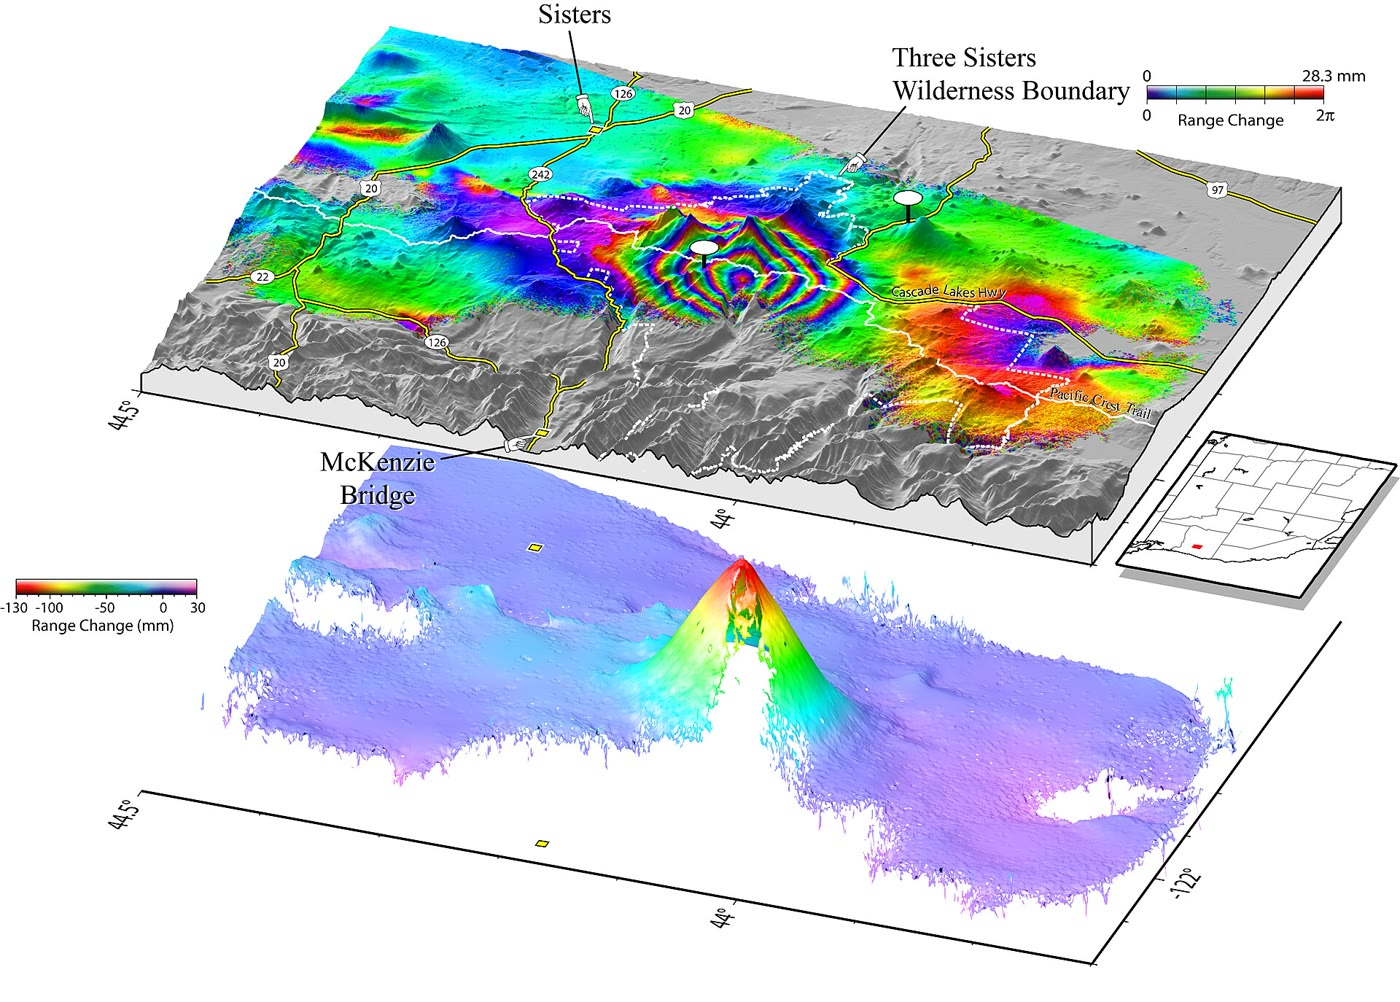
\includegraphics[width=0.86\linewidth]{images/book5/b3-three-sisters-insar.jpg}
\par\smallskip{\small Acima, o \omterm{def:b3:remote-sensing-gis:insar}{interferograma} do centro vulcânico Three Sisters,
Oregon, 1995--2001, sobreposto ao relevo: cada ciclo de cores corresponde a
\qty{28.3}{mm} de variação de distância, e o alvo de anéis concêntricos no
centro marca o soerguimento. Abaixo, os mesmos dados desdobrados e representados como
relevo: a distância diminui em até \qty{130}{mm} no centro. U.S.
Geological Survey (Wicks e outros, 2002), domínio
público.}\label{fig:b3:remote-sensing-gis:three-sisters}
\end{omfigure}
% ledger: photo:b3-three-sisters-insar, usgs:insar-fs

\begin{inthelab}[Uma estação de solo]
\begin{minipage}[t]{0.55\linewidth}\vspace{0pt}
Um satélite de imageamento registra muito mais do que consegue enviar enquanto passa
sobre o local que imageia. O radar de um satélite Sentinel-1 pode imagear
até meia hora de cada órbita e armazena seus dados a bordo, até
1410 gigabits; ele os envia ao solo em dois canais de 260 megabits por
segundo cada um, de modo que um armazenamento completo leva cerca de 45 minutos para ser esvaziado. Uma
estação de solo os recebe: à medida que o satélite surge acima do horizonte, a antena
gira para apontar para ele, acompanha-o pelo céu e o solta ao se pôr,
enquanto os operadores verificam se o fluxo chega completo. Os dados então
seguem para um centro de processamento, onde os ecos brutos se tornam imagens.
\end{minipage}\hfill
\begin{minipage}[t]{0.42\linewidth}\vspace{0pt}
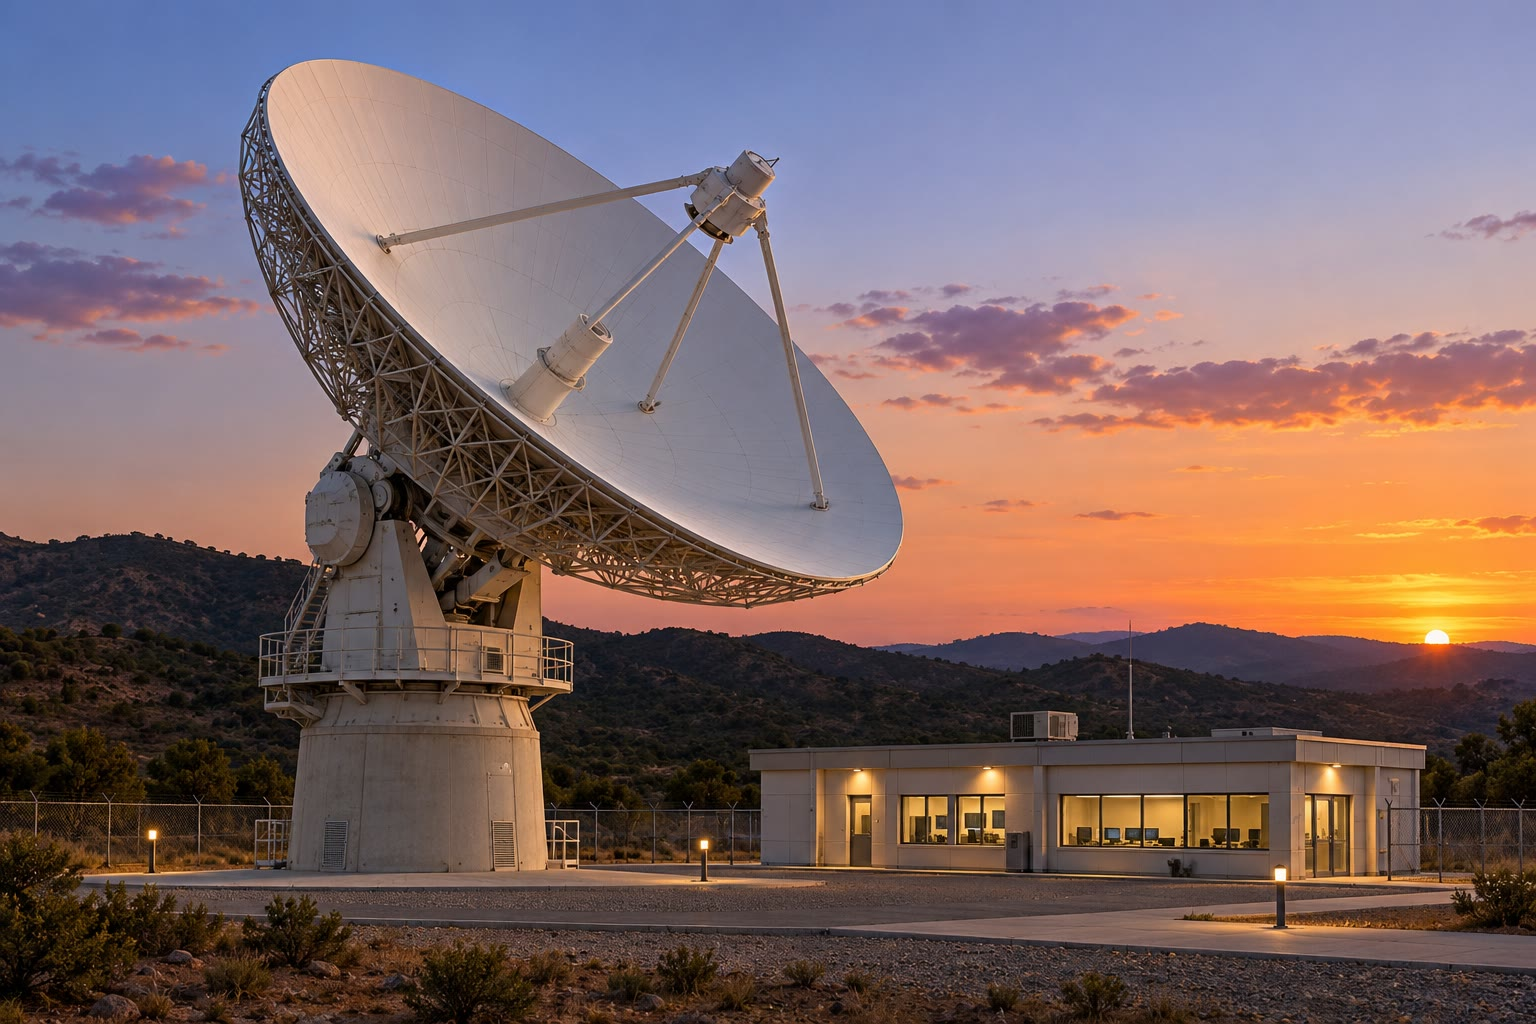
\includegraphics[width=\linewidth]{images/book5/ai/b3-ground-station.jpg}

{\scriptsize Uma estação de solo de satélite ao entardecer: uma grande antena de rastreamento e
seu prédio de operações (Ilustração gerada por IA.)}
\end{minipage}
\end{inthelab}
% ledger: esa:s1-downlink

\section{Sistemas de informação geográfica}\label{sec:b3:remote-sensing-gis:gis}

As imagens dos satélites, o modelo de elevação do terreno, o
mapa geológico, os poços e as estradas são camadas de um único
sistema de informação geográfica, que as armazena num sistema comum de coordenadas e
calcula com elas.

\begin{definition}[Dados matriciais e vetoriais]\label{def:b3:remote-sensing-gis:data-models}
Os \emph{dados matriciais}\index{dados matriciais} representam uma camada por uma grade de
células, cada uma guardando um valor: uma refletância, uma elevação, uma classe.
Os \emph{dados vetoriais}\index{dados vetoriais (SIG)} representam-na por pontos, linhas
e polígonos dados pelas coordenadas de seus vértices, cada um carregando uma
linha de atributos em uma tabela.
\end{definition}

\begin{omfigure}
\centering
\begin{tikzpicture}[x=0.5cm, y=0.5cm, font=\scriptsize]
\begin{scope}
\draw[black!40] (0,0) rectangle (10,7);
\fill[omSea!50, draw=omDef, thick] (3,4.5) ellipse (1.8 and 1.2);
\draw[omDef, very thick] (4.8,4.5) -- (7,3.5) -- (10,2);
\fill[red!70!black] (7,5.5) circle (0.14); \fill[red!70!black] (2,1.5) circle (0.14);
\node[anchor=south] at (5,7.1) {vetorial};
\node at (3,4.5) {lago};
\node[anchor=south west] at (7.1,5.6) {poço 1};
\node[anchor=south west] at (2.1,1.6) {poço 2};
\node[anchor=north east] at (9.9,2.2) {rio};
\end{scope}
\begin{scope}[xshift=6.5cm]
\foreach \i/\j in {1/4,2/4,3/4,4/4,2/3,3/3,2/5,3/5} {\fill[omSea!50] (\i,\j) rectangle ++(1,1);}
\foreach \i/\j in {5/4,6/3,7/3,8/2,9/2} {\fill[omDef!70] (\i,\j) rectangle ++(1,1);}
\foreach \i/\j in {7/5,2/1} {\fill[red!70!black] (\i,\j) rectangle ++(1,1);}
\draw[black!30, step=1] (0,0) grid (10,7);
\draw[black!40] (0,0) rectangle (10,7);
\node[anchor=south] at (5,7.1) {matricial};
\end{scope}
\end{tikzpicture}
\par\smallskip{\small O mesmo mapa como \omterm{def:b3:remote-sensing-gis:data-models}{dados vetoriais} (à esquerda: um polígono, uma linha
e dois pontos, exatos na posição, cada um com seus atributos) e como \omterm{def:b3:remote-sensing-gis:data-models}{dados matriciais}
(à direita: um valor por célula, o lago pelas células cujo centro fica
dentro dele, o rio e os poços pelas células que atravessam). Um dado matricial é fácil de
calcular, célula por célula; uma camada vetorial preserva formas e topologia em
qualquer escala.}\label{fig:b3:remote-sensing-gis:raster-vector}
\end{omfigure}

\begin{definition}[Georreferenciamento]\label{def:b3:remote-sensing-gis:georef}
O \emph{georreferenciamento}\index{georreferenciamento} é a atribuição de coordenadas de mapa
em uma projeção declarada a cada pixel de uma imagem ou a cada
vértice de um desenho, geralmente ajustando uma transformação a pontos de controle
no terreno cujas posições são conhecidas nos dois referenciais.
\end{definition}

Para um matricial com o norte para cima em um referencial projetado, a transformação é afim:
a célula na coluna $i$ e na linha $j$ tem seu canto em $E = E_0 + i\,\Delta$,
$N = N_0 - j\,\Delta$, sendo $\Delta$ o tamanho da célula. Uma imagem de satélite é
primeiro reamostrada numa grade desse tipo; camadas em projeções diferentes são
projetadas em uma única antes de serem combinadas.

\begin{method}[Declividade, orientação e relevo sombreado a partir de um modelo digital de elevação]\label{met:b3:remote-sensing-gis:slope}
Em uma grade de elevações $z_{i,j}$ de espaçamento $\Delta$ ($i$ para leste, $j$
para norte), estima-se o gradiente por diferenças centrais,
\[
\frac{\partial z}{\partial x} \approx \frac{z_{i+1,j} - z_{i-1,j}}{2\Delta} ,
\qquad
\frac{\partial z}{\partial y} \approx \frac{z_{i,j+1} - z_{i,j-1}}{2\Delta} .
\]
A \emph{declividade} é $S = \arctan|\nabla z|$; a \emph{orientação} é o
azimute da descida mais íngreme, a direção de $-\nabla z$, $A =
\operatorname{atan2}(-\partial z/\partial x, -\partial z/\partial y)$
medido no sentido horário a partir do norte. O \emph{relevo sombreado} para uma luz vinda do
azimute $A_0$ com ângulo zenital $Z$ é $\cos Z\cos S + \sin Z\sin S
\cos(A_0 - A)$, o cosseno do ângulo entre a luz e a normal
ao terreno, zerado onde for negativo.
\end{method}

A diferença central é exata para um plano e tem erro de
$\Delta^2 z'''/6$ em caso contrário; o relevo sombreado das Varden Hills no
volume do primeiro ano foi calculado dessa maneira, iluminado pelo noroeste. As derivadas
amplificam os erros da grade: um modelo com degraus entre suas linhas os mostra
como faixas em seu mapa de declividade.

\begin{definition}[Álgebra de mapas]\label{def:b3:remote-sensing-gis:map-algebra}
A \emph{álgebra de mapas}\index{álgebra de mapas} é o cálculo de uma nova
camada matricial célula por célula a partir de uma ou mais camadas da mesma grade: por
aritmética (o NDVI a partir de duas bandas), por comparação (as células mais íngremes que
\ang{15}), por operações lógicas (e, ou, não), ou a partir de uma vizinhança
da célula (a declividade).
\end{definition}

\begin{definition}[Zona de influência; sobreposição]\label{def:b3:remote-sensing-gis:operations}
A \emph{zona de influência}\index{zona de influência (SIG)} de um elemento à distância $d$ é
a região do mapa a menos de $d$ dele. Uma
\emph{sobreposição}\index{sobreposição (SIG)} combina duas ou mais camadas da
mesma área em uma só, cada lugar do resultado carregando os atributos de
todas elas; a seleção dos lugares que atendem a várias condições ao mesmo
tempo é o uso mais comum.
\end{definition}

\begin{omfigure}
\centering
\begin{tikzpicture}
\begin{groupplot}[group style={group size=2 by 2, horizontal sep=2.0cm, vertical sep=1.5cm},
  width=0.43\linewidth, axis equal image, enlargelimits=false,
  xmin=0, xmax=10, ymin=0, ymax=8,
  tick label style={font=\scriptsize}, label style={font=\small}, title style={font=\small}]
\nextgroupplot[title={(a) declividade (graus)}, ylabel={norte (km)}, colormap/viridis,
  point meta min=0, point meta max=24, colorbar right,
  colorbar style={width=0.18cm, ytick={0,5,10,15,20}, tick label style={font=\tiny}, axis equal=false}]
\addplot[matrix plot*, mesh/cols=101, point meta=explicit] table[x=x, y=y, meta=slope] {figdata/out/bachelor-3-varden_gis-grid.dat};
\addplot[white, thick] table {figdata/out/shared-region-river.dat};
\nextgroupplot[title={(b) orientação},
  colormap={aspect}{rgb255=(220,20,30) rgb255=(240,200,0) rgb255=(30,170,60) rgb255=(30,90,220) rgb255=(220,20,30)},
  point meta min=0, point meta max=360, colorbar right,
  colorbar style={width=0.18cm, ytick={0,90,180,270,360}, yticklabels={N,L,S,O,N}, tick label style={font=\tiny}, axis equal=false}]
\addplot[matrix plot*, mesh/cols=101, point meta=explicit] table[x=x, y=y, meta=aspect] {figdata/out/bachelor-3-varden_gis-grid.dat};
\addplot[black, thick] table {figdata/out/shared-region-river.dat};
\nextgroupplot[title={(c) duas camadas}, xlabel={leste (km)}, ylabel={norte (km)},
  colormap={lay}{rgb255=(245,245,245) rgb255=(150,150,150) rgb255=(225,195,140) rgb255=(120,70,20)},
  colormap access=piecewise constant, point meta min=-0.5, point meta max=3.5,
  legend columns=2, legend style={font=\tiny, at={(0.5,-0.3)}, anchor=north, /tikz/every even column/.append style={column sep=4pt}}]
\addplot[matrix plot*, mesh/cols=101, point meta=explicit, forget plot] table[x=x, y=y, meta=layers] {figdata/out/bachelor-3-varden_gis-grid.dat};
\addplot[omDef, thick, forget plot] table {figdata/out/shared-region-river.dat};
\addlegendimage{area legend, fill={rgb,255:red,150;green,150;blue,150}, draw=black!40}
\addlegendentry{mais íngreme que \ang{15}}
\addlegendimage{area legend, fill={rgb,255:red,225;green,195;blue,140}, draw=black!40}
\addlegendentry{folhelho}
\addlegendimage{area legend, fill={rgb,255:red,120;green,70;blue,20}, draw=black!40}
\addlegendentry{ambos}
\nextgroupplot[title={(d) sobreposição}, xlabel={leste (km)},
  colormap={cls}{rgb255=(245,245,245) rgb255=(225,195,140) rgb255=(190,150,90) rgb255=(200,20,30)},
  colormap access=piecewise constant, point meta min=-0.5, point meta max=3.5,
  legend columns=2, legend style={font=\tiny, at={(0.5,-0.3)}, anchor=north, /tikz/every even column/.append style={column sep=4pt}}]
\addplot[matrix plot*, mesh/cols=101, point meta=explicit, forget plot] table[x=x, y=y, meta=class] {figdata/out/bachelor-3-varden_gis-grid.dat};
\addplot[omDef, thick, forget plot] table {figdata/out/shared-region-river.dat};
\addplot[black, thin, dashed, unbounded coords=jump] table[x=x, y=y] {figdata/out/bachelor-3-varden_gis-buffer.dat};
\addlegendentry{zona de influência de \qty{1}{km}}
\addlegendimage{area legend, fill={rgb,255:red,225;green,195;blue,140}, draw=black!40}
\addlegendentry{folhelho}
\addlegendimage{area legend, fill={rgb,255:red,190;green,150;blue,90}, draw=black!40}
\addlegendentry{folhelho na zona de influência}
\addlegendimage{area legend, fill={rgb,255:red,200;green,20;blue,30}, draw=black!40}
\addlegendentry{selecionado}
\end{groupplot}
\end{tikzpicture}
\par\smallskip{\small Uma sessão de SIG nas Varden Hills, a partir do seu modelo de elevação
numa grade de \qty{100}{m}. (a)~A declividade, até \ang{23} nas
encostas do vale; (b)~a orientação, a direção para a qual o terreno está voltado, os dois lados do
rio voltados um para o outro; (c)~duas camadas, as células mais íngremes que \ang{15}
e o afloramento do folhelho jurássico; (d)~a \omterm{def:b3:remote-sensing-gis:operations}{sobreposição} delas com a
\omterm{def:b3:remote-sensing-gis:operations}{zona de influência} de \qty{1}{km} do rio (tracejada): os \qty{0.32}{km^2} de
folhelho íngreme acima do rio, uma primeira triagem de terrenos que
podem deslizar.}\label{fig:b3:remote-sensing-gis:varden}
\end{omfigure}

A figura acima percorre toda a cadeia: a \omterm{def:b3:remote-sensing-gis:map-algebra}{álgebra de mapas} sobre a grade de elevação
fornece a declividade e a orientação; uma comparação transforma a declividade
numa camada de células íngremes; o mapa geológico fornece o folhelho; a \omterm{def:b3:remote-sensing-gis:operations}{zona de
influência} do rio fornece uma terceira camada; a interseção delas, uma \omterm{def:b3:remote-sensing-gis:operations}{sobreposição}
com o \emph{e} lógico, deixa 32 células das 8181. A resposta vale apenas o que valem as
camadas: numa grade mais grossa, as declividades saem mais suaves e passam menos células.

\begin{definition}[Classificação supervisionada; matriz de confusão]\label{def:b3:remote-sensing-gis:classification}
Uma \emph{classificação supervisionada}\index{classificação supervisionada}
atribui cada pixel de uma imagem a uma de um conjunto de classes, a partir de regras ou
estatísticas aprendidas em pixels de treinamento cuja classe é conhecida em campo.
Sua \emph{matriz de confusão}\index{matriz de confusão} conta, para um conjunto separado
de pixels de referência, quantos de cada classe verdadeira foram atribuídos a cada
classe: $n_{ij}$ pixels classificados como $i$ pertencem, na verdade, a $j$.
\end{definition}

A diagonal contém os pixels classificados corretamente. Com $N$ pixels de referência,
a \emph{acurácia global} é $\sum_i n_{ii}/N$. A \emph{acurácia do
usuário} de uma classe, $n_{ii}$ sobre o total de sua linha, é a chance de que um
pixel que o mapa chama de $i$ seja $i$; sua \emph{acurácia do produtor}, $n_{ii}$
sobre o total de sua coluna, é a chance de que um $i$ verdadeiro tenha sido mapeado como $i$. O
coeficiente \emph{kappa} compara a acurácia global $p_o$ com a
acurácia $p_e = \sum_i (\text{lin}_i)(\text{col}_i)/N^2$ que a atribuição aleatória
com os mesmos totais alcançaria: $\kappa = (p_o - p_e)/(1 -
p_e)$.

\begin{center}
\small
\begin{tabular}{l|ccc|c}
\hline
classificado \textbackslash{} referência & água & floresta & rocha exposta & total \\
\hline
água & 45 & 2 & 0 & 47 \\
floresta & 3 & 38 & 7 & 48 \\
rocha exposta & 0 & 5 & 30 & 35 \\
\hline
total & 48 & 45 & 37 & 130 \\
\hline
\end{tabular}
\end{center}

Neste exemplo fictício, 113 de 130 pixels estão corretos, uma acurácia
global de \qty{86.9}{\percent}. A floresta tem acurácia do usuário de
$38/48 = \qty{79}{\percent}$, mas acurácia do produtor de $38/45 =
\qty{84}{\percent}$: sete pixels de rocha exposta, talvez em sombra, foram
chamados de floresta. A atribuição aleatória alcançaria $p_e = 0.338$, e $\kappa =
0.80$.

\section{Exercícios}

\begin{exercise}[$\star$]\label{exo:b3:remote-sensing-gis:1}
Um campo tem refletâncias de 0.06 na banda do vermelho e 0.42 no
infravermelho próximo de um imageador; um campo arado vizinho tem 0.21 e
0.28. Calcule o NDVI de ambos e diga o que cada valor sugere.
\end{exercise}

\begin{exercise}[$\star$]\label{exo:b3:remote-sensing-gis:2}
O imageador Landsat~8 cobre uma faixa de \qty{185}{km} de largura, com pixels de \qty{30}{m}
pixels, e sua banda pancromática com pixels de \qty{15}{m}. (a)~Quantos
pixels uma linha atravessando a faixa contém em cada caso? (b)~Quantos níveis
dão 12 bits, e 8 bits? (c)~Qual é o \omterm{def:b3:remote-sensing-gis:resolutions}{tempo de revisita} do Landsat~8
sozinho, e dos Landsats 8 e 9 juntos?
\end{exercise}

\begin{exercise}[$\star$]\label{exo:b3:remote-sensing-gis:3}
(a)~Em um \omterm{def:b3:remote-sensing-gis:insar}{interferograma} do Sentinel-1 ($\lambda = \qty{5.55}{cm}$) de uma
bacia em subsidência, seis franjas separam a borda estável do centro.
Qual é a variação da \omterm{def:b3:remote-sensing-gis:insar}{linha de visada} no centro? (b)~Quanto valeria uma franja
para um satélite mais antigo de comprimento de onda \qty{5.66}{cm}?
\end{exercise}

\begin{exercise}[$\star$]\label{exo:b3:remote-sensing-gis:4}
Um altímetro a laser está a \qty{500}{km} acima do solo. (a)~Quanto tempo um
pulso leva para retornar? (b)~Se cada fóton for cronometrado com \qty{800}{ps}, qual
é a precisão de uma medida de distância?
\end{exercise}

\begin{exercise}[$\star\star$]\label{exo:b3:remote-sensing-gis:5}
Um pixel da banda~10 do Landsat~8 (considere $\lambda = \qty{10.9}{\micro\metre}$)
tem, após a \omterm{def:b3:remote-sensing-gis:atm-correction}{correção atmosférica}, uma radiância espectral de
\qty{9.0}{W.m^{-2}.sr^{-1}.\micro\metre^{-1}}. (a)~Calcule a
\omterm{def:b3:remote-sensing-gis:brightness}{temperatura de brilho}. (b)~A superfície é um campo de gramíneas de emissividade 0.98: qual é
sua temperatura cinética?
\end{exercise}

\begin{exercise}[$\star\star$]\label{exo:b3:remote-sensing-gis:6}
O radar do Sentinel-1 voa a \qty{693}{km} de altura, com uma antena de \qty{12.3}{m}
de comprimento em $\lambda = \qty{5.55}{cm}$. (a)~Desprezando a curvatura da
Terra, calcule a distância oblíqua até um ponto visto com incidência de
\ang{35}. (b)~Que resolução azimutal teria ali uma antena real desse comprimento, e
o que dá a abertura sintética? (c)~Qual é o comprimento da
abertura sintética?
\end{exercise}

\begin{exercise}[$\star\star$]\label{exo:b3:remote-sensing-gis:7}
Uma janela $3\times3$ de um modelo digital de elevação com células de \qty{30}{m}
lê, com o norte no topo,
\[
\begin{matrix} 412 & 418 & 425 \\ 405 & 410 & 418 \\ 398 & 401 & 409 \end{matrix}
\qquad (\unit{m}).
\]
Por diferenças centrais na célula central, calcule a declividade, a
orientação e o sombreamento para uma luz vinda do noroeste, \ang{45} acima do
horizonte.
\end{exercise}

\begin{exercise}[$\star\star$]\label{exo:b3:remote-sensing-gis:8}
Um mapa de cobertura do solo é verificado contra 160 pixels de referência (linhas: o mapa;
colunas: a verdade; classes água, floresta, cultivos, cidade):
\[
\begin{pmatrix} 48 & 3 & 1 & 0 \\ 4 & 37 & 6 & 1 \\ 2 & 5 & 29 & 2 \\ 0 & 1 & 2 & 19 \end{pmatrix} .
\]
Calcule a acurácia global, as acurácias do usuário e do produtor de cada
classe, e o kappa. Qual classe é perdida com mais frequência?
\end{exercise}

\begin{exercise}[$\star\star$]\label{exo:b3:remote-sensing-gis:9}
Um pixel térmico de \qty{100}{m} contém um fluxo de lava recente a \qty{1443}{K}
que cobre \qty{4}{\percent} dele; o restante é solo a \qty{290}{K}; considere
ambos como corpos negros. (a)~Calcule a \omterm{def:b3:remote-sensing-gis:brightness}{temperatura de brilho} do pixel
em \qty{10.9}{\micro\metre} e compare-a com a temperatura média.
(b)~Calcule a razão entre as radiâncias de corpo negro da lava e do
solo em \qty{2.2}{\micro\metre}, e a \omterm{def:b3:remote-sensing-gis:brightness}{temperatura de brilho} do
pixel nesse comprimento de onda. Qual banda detecta melhor a lava?
\end{exercise}

\begin{exercise}[$\star\star\star$]\label{exo:b3:remote-sensing-gis:10}
Dois \omterm{def:b3:remote-sensing-gis:insar}{interferogramas} da mesma deformação são obtidos a partir de duas passagens, uma
com o satélite a L do terreno e outra com ele a O,
ambos com incidência de \ang{35}. Em um ponto, a
\omterm{def:b3:remote-sensing-gis:insar}{linha de visada} encurta \qty{64}{mm} na primeira e \qty{38}{mm} na
segunda. Supondo que não haja movimento norte--sul, calcule os deslocamentos vertical e
leste. Por que uma única passagem não basta?
\end{exercise}

\begin{exercise}[$\star\star\star$]\label{exo:b3:remote-sensing-gis:11}
O \omterm{def:b3:remote-sensing-gis:insar}{desdobramento de fase} falha onde a fase salta mais de $\pi$ entre
pixels vizinhos. (a)~Mostre que a \omterm{def:b3:remote-sensing-gis:insar}{linha de visada} deve variar menos de
$\lambda/4$ de um pixel para o seguinte, \qty{13.9}{mm} para
o Sentinel-1. (b)~Para uma fonte de Mogi em $z_0 = \qty{4}{km}$, com $\Delta V =
\qty{e7}{m^3}$ e $\nu = 0.25$, vista na vertical, mostre que o gradiente mais acentuado
de $u_z$ está em $r = z_0/2$ e calcule-o. (c)~Qual é o maior tamanho de pixel que
mantém as franjas resolvíveis?
\end{exercise}

\begin{exercise}[$\star\star\star$]\label{exo:b3:remote-sensing-gis:12}
(a)~Mostre que o NDVI está entre $-1$ e $+1$ para refletâncias não negativas, e que ele
não muda quando ambas as refletâncias são
multiplicadas pelo mesmo fator. (b)~A grama tem refletâncias de 0.051 (vermelho)
e 0.502 (infravermelho próximo). Uma imagem não corrigida acrescenta uma radiância de caminho
equivalente a 0.03 no vermelho e 0.01 no infravermelho próximo. Calcule o
NDVI com e sem essa correção. (c)~O que isso implica para um mapa de NDVI
feito a partir de imagens não corrigidas em um dia com névoa?
\end{exercise}

\section{Problema: uma encosta inchando no monte Halvren}

\begin{problem}[{Problema de fim de semana --- vegetação, calor e um radar
interferograma sobre um vulcão inventado}]
\label{pb:b3:remote-sensing-gis:1}
O monte Halvren, um vulcão inventado, expeliu fluxos de lava em 1890, 1960
e 2005 sobre suas encostas florestadas. Um campo de fumarolas exala vapor em seu cume.
Dados de satélite de um ano recente são apresentados a seguir.

\medskip\noindent\textbf{Parte I --- Vegetação sobre os fluxos de lava.} Refletâncias corrigidas
nas bandas do vermelho e do infravermelho próximo:
\begin{center}
\small
\begin{tabular}{lcccc}
\hline
superfície & floresta & fluxo de 1890 & fluxo de 1960 & fluxo de 2005 \\
\hline
vermelho & 0.04 & 0.07 & 0.11 & 0.12 \\
infravermelho próximo & 0.38 & 0.30 & 0.21 & 0.14 \\
\hline
\end{tabular}
\end{center}
\begin{enumerate}
\item Calcule o NDVI das quatro superfícies.
\item Ordene os fluxos pela \omterm{def:b3:deformation-mechanisms:recrystallisation}{recuperação} de sua vegetação. A
  ordem coincide com a das idades deles?
\item Por que o NDVI do fluxo de 2005 não é zero, embora quase
  nada cresça sobre ele?
\item Por que o NDVI é mais confiável do que a refletância do infravermelho próximo
  isoladamente nas encostas íngremes e irregularmente iluminadas de um vulcão?
\end{enumerate}

\medskip\noindent\textbf{Parte II --- O campo de fumarolas.} Na banda térmica
(considere $\lambda = \qty{10.9}{\micro\metre}$) a radiância corrigida de
um pixel de \qty{100}{m} do platô do cume, afastado das fumarolas, é
\qty{8.40}{W.m^{-2}.sr^{-1}.\micro\metre^{-1}}, e a do pixel sobre
o campo de fumarolas \qty{9.95}{W.m^{-2}.sr^{-1}.\micro\metre^{-1}}.
\begin{enumerate}[resume]
\item Calcule as \omterm{def:b3:remote-sensing-gis:brightness}{temperaturas de brilho} dos dois pixels.
\item A rocha do platô tem emissividade de 0.97. Qual é a sua temperatura
  cinética?
\item As fumarolas e o solo quente ao redor delas estão a
  \qty{370}{K}. Tratando-os, bem como o restante do pixel, como corpos negros,
  com o restante na radiância do platô, qual fração do pixel eles cobrem
  e qual é essa área?
\item Por que a temperatura média ponderada pela área do pixel fica abaixo
  de sua \omterm{def:b3:remote-sensing-gis:brightness}{temperatura de brilho}?
\end{enumerate}

\medskip\noindent\textbf{Parte III --- O interferograma.} Duas
imagens do Sentinel-1 ($\lambda = \qty{5.55}{cm}$, incidência de \ang{35}, satélite a L)
obtidas com 48 dias de intervalo mostram um padrão de olho de boi na encosta leste. Do
terreno estável até o centro do padrão conta-se cinco franjas completas e
quatro décimos de uma sexta, todas no sentido do movimento em direção ao
satélite.
\begin{enumerate}[resume]
\item Por que as duas imagens devem ser obtidas a partir de posições quase iguais, e
  quantos ciclos orbitais de um satélite as separam?
\item Calcule a variação da \omterm{def:b3:remote-sensing-gis:insar}{linha de visada} no centro.
\item No centro, o solo se move apenas verticalmente. Calcule o soerguimento
  ali.
\item Explique por que o padrão não é circular e de qual lado, L ou O, as
  franjas estão mais concentradas.
\item Ao longo da linha norte--sul que passa pelo centro, a variação da \omterm{def:b3:remote-sensing-gis:insar}{linha de visada}
  cai à metade de seu valor central a \qty{3.4}{km} do
  centro. Por que usar essa linha, e qual profundidade ela fornece para uma fonte
  de Mogi?
\item Quantas franjas separam o centro desse ponto de meia altura?
\item O vapor d'água no ar pode atrasar as ondas de radar de modo diferente nas duas
  datas e produzir franjas próprias. Como um segundo \omterm{def:b3:remote-sensing-gis:insar}{interferograma},
  de outro par de datas, ajudaria a distinguir os dois efeitos?
\end{enumerate}

\medskip\noindent\textbf{Parte IV --- O volume.} Considere $\nu = 0.25$.
\begin{enumerate}[resume]
\item A partir de $u_z(0) = (1 - \nu)\Delta V/(\pi z_0^2)$, calcule a variação de volume
  da fonte.
\item Expresse-a como taxa média por dia e por ano ao longo dos 48 dias.
\item Calcule o maior deslocamento horizontal e onde ele ocorre.
\item Se o reservatório fosse uma esfera de raio $z_0/3$, qual seria o seu volume e
  que fração dele a variação representa?
\item O tamanho finito de uma esfera de raio $z_0/3$ altera o soerguimento em cerca de
  \qty{3}{\percent}. Isso altera de modo apreciável a resposta à questão~16, dada a
  precisão da contagem de franjas?
\item Que outra observação, das Partes I e II ou feita no terreno, apoiaria a
  interpretação de um reservatório se enchendo?
\item Dê a variação de volume do reservatório sob o monte Halvren, em milhões de
  metros cúbicos, com dois algarismos significativos.
\end{enumerate}
\end{problem}
% ledger: nasa:ndvi, esa:s1-sar, esa:s1-orbit, esa:s1-iw, dmodels:mogi, dmodels:mogi-radial, const:h, const:c, const:kB
